\documentclass[12pt,a4paper]{article}
\usepackage[T2A]{fontenc}
\usepackage[utf8]{inputenc}
\usepackage[ukrainian]{babel}
\usepackage[left=2.5cm,right=2cm,top=2cm,bottom=2.5cm]{geometry}
\usepackage{graphicx}
\usepackage{float}
\usepackage{booktabs}
\usepackage{array}
\usepackage{amsmath}
\usepackage[labelsep=colon]{caption}
\usepackage{enumitem}
\usepackage{fancyvrb}
\usepackage{indentfirst}
\usepackage{tikz}
\usetikzlibrary{positioning,arrows.meta,shapes.geometric}

\graphicspath{{figures/}}
\fvset{fontsize=\small,frame=single,framesep=2mm}
\setlist[enumerate]{leftmargin=*}
\setlength{\parskip}{0.3em}
\setlength{\emergencystretch}{3em}

% Титульна сторінка: #1 — номер лабораторної роботи
\newcommand{\labtitlepage}[1]{%
\begin{titlepage}
\begin{center}
\large
Міністерство освіти і науки України\\
Національний університет ``Львівська політехніка''\\
Кафедра прикладної математики
\vspace*{\fill}

{\LARGE Звіт}\\[0.5em]
{\Large про виконання лабораторної роботи №#1}\\[0.5em]
{\Large з курсу «Основи інженерії даних»}
\vspace*{\fill}
\end{center}
\begin{flushright}
\begin{minipage}{0.4\textwidth}
\large
Виконала:\\
студентка групи ПМІД-11\\
Мазур Д. М.\\[1.5em]
Перевірив:\\
Алєксєєв В. І.
\end{minipage}
\end{flushright}
\vspace*{\fill}
\begin{center}
\large Львів — 2026
\end{center}
\end{titlepage}
\setcounter{page}{2}}

\newcommand{\rsec}[1]{\par\medskip\noindent\textbf{#1}\ }

\begin{document}
\labtitlepage{4}

\rsec{Тема:} Розподілена обробка даних та паралелізм з Apache Spark.

\rsec{Мета роботи:} Оволодіти концепціями розподілених обчислень, зосереджуючись на тому, як розподіл даних та операції перетасування (shuffle) впливають на продуктивність і масштабованість паралельних алгоритмів. Проаналізувати продуктивність паралельного алгоритму за допомогою закону Амдала та обміркувати, як обробляти асиметрію даних (data skew).

\rsec{Постановка задачі:} Проаналізувати великий набір даних лог-файлу, щоб обчислити середню тривалість сеансу користувача.

\rsec{Завдання до роботи:}
\begin{enumerate}
  \item Підготувати набір даних Parquet зі схемою (\texttt{user\_id}: STRING, \texttt{session\_id}: STRING, \texttt{event\_timestamp}: LONG, мілісекунди).
  \item Налаштувати Spark для роботи на кластері з X виконавцями та Y ядрами на виконавця.
  \item Реалізувати алгоритм 1 «наївне перетасування» (налаштування за замовчуванням), виміряти час і метрики перетасування.
  \item Реалізувати алгоритм 2 «оптимізоване перетасування» з явним розподілом даних перед агрегацією.
  \item Оцінити максимально досяжне прискорення за законом Амдала на основі виміряного часу.
  \item Проаналізувати, як виявити та пом'якшити асиметрію даних, якщо один користувач становить 90\% усіх сеансів.
\end{enumerate}

\rsec{Хід виконання роботи:}
\begin{enumerate}
  \item \textbf{Середовище та налаштування.} Використано PySpark 4.0.4 (Java 17) у локальному режимі. Режим \texttt{local[Y]} відповідає одному виконавцю (X = 1), що працює в JVM драйвера, з Y = 4 ядрами, тобто 4 паралельними задачами. На реальному кластері ці значення задаються параметрами \texttt{spark.executor.instances = X} і \texttt{spark.executor.cores = Y}, а загальна кількість паралельних задач дорівнює X\(\times\)Y. Пам'ять драйвера становить 4~GB. Решта параметрів за замовчуванням: \texttt{spark.sql.shuffle.partitions = 200}, увімкнено Adaptive Query Execution (AQE).

  \item \textbf{Підготовка даних.} Скрипт \texttt{lab4\_db/generate\_data.py} генерує лог засобами самого Spark (\texttt{spark.range}, без створення даних у Python). Згенеровано 400\,000 сесій для 50\,000 користувачів. Кожна сесія належить одному користувачу і містить від 2 до 20 подій у межах до 2 годин. Разом вийшло 4\,397\,801 подія. Події записано у 16 файлів Parquet із round-robin перемішуванням, тому події однієї сесії розкидані по різних файлах, як у реальних логах. Другий набір \texttt{logs\_skewed.parquet} має таку саму структуру, але 90\% сесій у ньому належать одному користувачу \texttt{user\_whale}.

  \item \textbf{Алгоритм розрахунку.} Кроки 2--4 завдання реалізовано однією функцією: групування за (\texttt{user\_id}, \texttt{session\_id}), тривалість як MAX\(-\)MIN мітки часу, потім загальне середнє:
\begin{Verbatim}
def session_durations(df):
    return df.groupBy("user_id", "session_id").agg(
        (F.max("event_timestamp") - F.min("event_timestamp"))
        .alias("duration_ms"))

def average_session_duration(df):
    return session_durations(df).agg(F.avg("duration_ms")).collect()[0][0]
\end{Verbatim}
  Вхідні дані попередньо кешуються в пам'яті (\texttt{df.cache().count()}), тому читання з диска не входить у виміряний час. Кожен варіант виконується раз для прогріву, потім тричі, і береться медіана. Метрики перетасування (обсяг shuffle write/read, кількість stages і tasks) зчитуються з REST API Spark UI для групи задач кожного запуску, а кількість операцій Exchange — з фізичного плану запиту.

  \item \textbf{Порівняння стратегій розподілу.} Порівняно три варіанти:
  \begin{itemize}
    \item \emph{Стратегія A, «високе перетасування»} (алгоритм 1): \texttt{df.repartition(200)} без ключа перед \texttt{groupBy}. Round-robin перемішує \emph{всі} сирі події, після чого \texttt{groupBy} виконує ще одне перетасування за ключем;
    \item \emph{Default}: просто \texttt{groupBy} з налаштуваннями за замовчуванням, для довідки;
    \item \emph{Стратегія B, «низьке перетасування»} (алгоритм 2): \texttt{df.repartition(4, 'user\_id', 'session\_id')}. Це hash-розподіл за ключем групування, кількість партицій дорівнює кількості ядер. Дані вже розподілені за потрібним ключем, тому \texttt{groupBy} не потребує другого Exchange.
  \end{itemize}

\begin{table}[H]
\centering
\caption{Порівняння стратегій розподілу (4 ядра, 4\,397\,801 подія)}
\label{tab:strat}
\begin{tabular}{lrrrrr}
\toprule
Стратегія & Час, с & Shuffle, MB & Записів & Exchange & Tasks \\
\midrule
A: repartition(200) & 3.66 & 248.3 & 8\,659\,076 & 2 & 209 \\
Default groupBy & 0.55 & 43.7 & 1\,411\,222 & 1 & 9 \\
B: repartition(4, ключі) & 0.53 & 97.7 & 4\,397\,805 & 1 & 9 \\
\bottomrule
\end{tabular}
\end{table}

Усі стратегії дали однакову середню тривалість сесії: 2\,787\,661~мс \(\approx\) 46.5~хв. Стратегія B виявилася в \textbf{6.8 раза швидшою} за стратегію A і перетасувала в 2.5 раза менше даних (97.7 проти 248.3~MB). У стратегії A кожна подія проходить через мережу двічі (8.66 млн записів у shuffle на 4.40 млн подій), а 200 дрібних задач додають накладні витрати на планування.

  Варіант Default записав у shuffle найменше даних (43.7~MB) завдяки \emph{частковій агрегації} (map-side combine): MAX і MIN обчислюються ще до перетасування. Тому явний \texttt{repartition} за ключем виправданий, коли розподіл використовують кілька подальших операцій або потрібен контроль кількості партицій.

  \item \textbf{Моделювання продуктивності за законом Амдала.} Стратегію B виміряно на 1, 2, 4 і 8 ядрах (кількість партицій дорівнює кількості ядер). Закон Амдала описує час виконання на \(n\) ядрах як суму послідовної та паралельної частин:
\begin{equation*}
T(n) = T_{\text{seq}} + \frac{T_{\text{par}}}{n}, \qquad
S(n) = \frac{T(1)}{T(n)} = \frac{1}{(1-p) + p/n}, \qquad
S_{\max} = \lim_{n\to\infty} S(n) = \frac{1}{1-p},
\end{equation*}
  де \(p = T_{\text{par}} / (T_{\text{seq}} + T_{\text{par}})\) — паралельна частка. Модель лінійна відносно \(1/n\), тому \(T_{\text{seq}}\) і \(T_{\text{par}}\) знайдено методом найменших квадратів за чотирма вимірюваннями:
\begin{equation*}
T(n) = 0.157 + \frac{1.618}{n}\ \text{с}, \qquad p = \frac{1.618}{0.157 + 1.618} = 0.912, \qquad S_{\max} = \frac{1}{1 - 0.912} \approx 11.3.
\end{equation*}
  Додатково обчислено метрику Карпа--Флатта \(e = \dfrac{1/S - 1/n}{1 - 1/n}\), тобто експериментально визначену послідовну частку (табл.~\ref{tab:amdahl}, рис.~\ref{fig:amdahl}).

\begin{table}[H]
\centering
\caption{Масштабування стратегії B за кількістю ядер}
\label{tab:amdahl}
\begin{tabular}{rrrrrr}
\toprule
\(n\) & \(T(n)\), с & \(S\) виміряне & \(S\) за Амдалом & Ефективність \(S/n\) & Карп--Флатт \(e\) \\
\midrule
1 & 1.761 & 1.00 & 1.00 & 1.00 & -- \\
2 & 1.007 & 1.75 & 1.84 & 0.87 & 0.144 \\
4 & 0.533 & 3.30 & 3.16 & 0.83 & 0.070 \\
8 & 0.360 & 4.89 & 4.94 & 0.61 & 0.091 \\
\bottomrule
\end{tabular}
\end{table}

\begin{figure}[H]
\centering
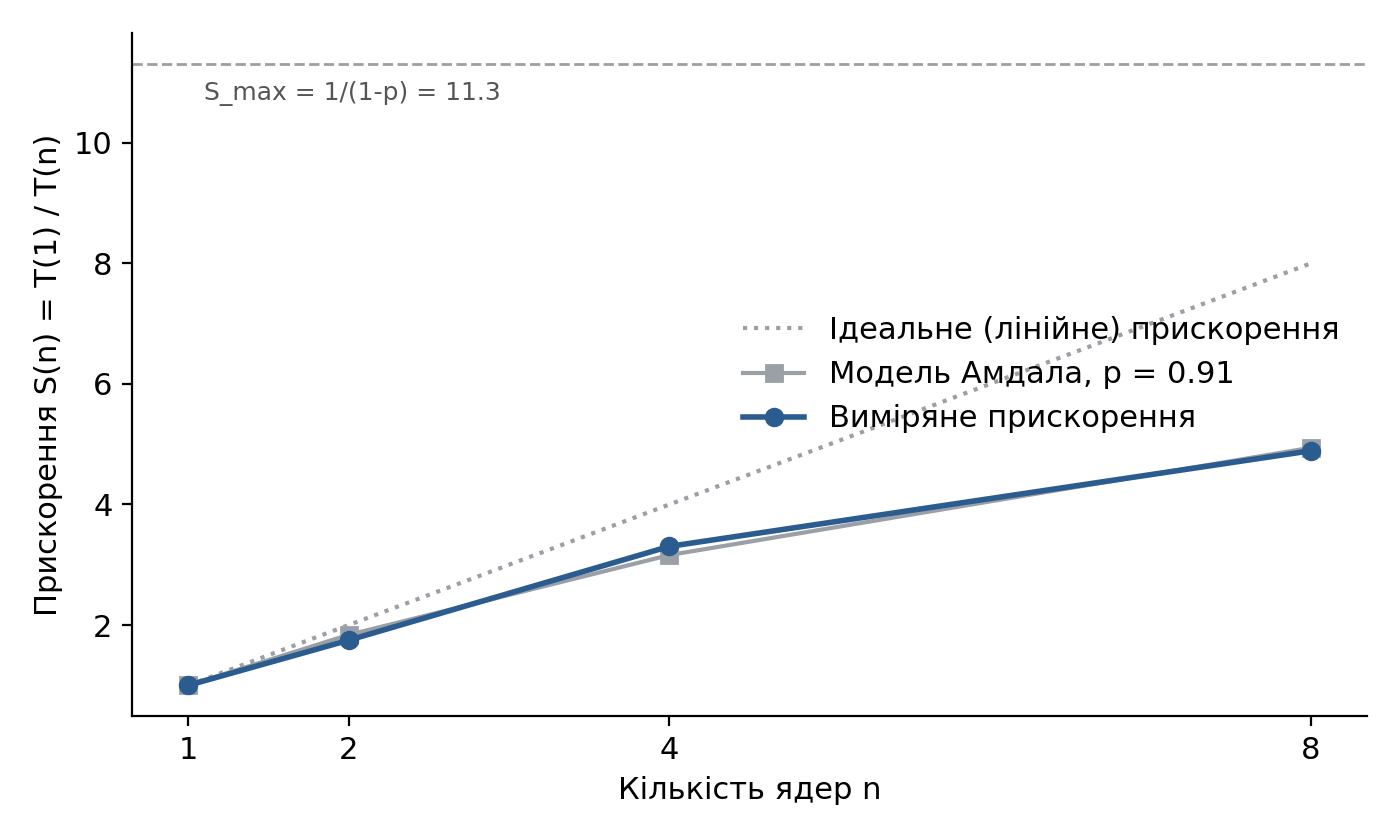
\includegraphics[width=0.62\textwidth]{lab4_amdahl.png}
\caption{Виміряне прискорення порівняно з моделлю Амдала та ідеальним лінійним прискоренням}
\label{fig:amdahl}
\end{figure}

  \emph{Послідовні компоненти}, які не масштабуються з ядрами: планування запиту та кодогенерація на драйвері, планування задач, фінальна агрегація AVG в одній партиції, \texttt{collect()} результату на драйвер, бар'єри синхронізації між stages. \emph{Паралельні компоненти}: сканування кешованих партицій, часткова агрегація MAX/MIN, запис і читання shuffle-блоків, агрегація за ключем. Модель узгоджується з вимірюваннями з точністю до 5\%. Оцінка \(p\) чутлива до шуму: в окремих запусках вона становила 0.76--0.91, тому \(S_{\max}\) слід розглядати як орієнтир (від 4 до 11).

  \item \textbf{Аналіз асиметрії даних (data skew).} Для набору \texttt{logs\_skewed.parquet} користувач \texttt{user\_whale} має 360\,040 із 400\,000 сесій (90.0\%), а наступні за ним користувачі — лише по 6 сесій. \emph{Виявлення} перекосу виконано двома способами: розподілом кількості сесій за \texttt{user\_id} (top-N і частка лідера) та розміром кожної партиції після розподілу (\texttt{spark\_partition\_id}). У Spark UI перекіс видно як задачу-«відстаючу» (straggler), тривалість і Shuffle Read якої значно більші за медіану по stage. Порівняно три варіанти розподілу (табл.~\ref{tab:skew}, рис.~\ref{fig:skew}).

\begin{table}[H]
\centering
\caption{Вплив перекосу та способів його пом'якшення (4 партиції)}
\label{tab:skew}
\begin{tabular}{lrrr}
\toprule
Варіант розподілу & Найбільша партиція & max / медіана & Час, с \\
\midrule
Наївний: за \texttt{user\_id} & 92.4\% & 36.6 & 1.21 \\
Fix 1: за (\texttt{user\_id}, \texttt{session\_id}) & 25.1\% & 1.0 & 0.48 \\
Fix 2: salting, 32 значення солі & 39.2\% & 1.6 & 0.71 \\
\bottomrule
\end{tabular}
\end{table}

\begin{figure}[H]
\centering
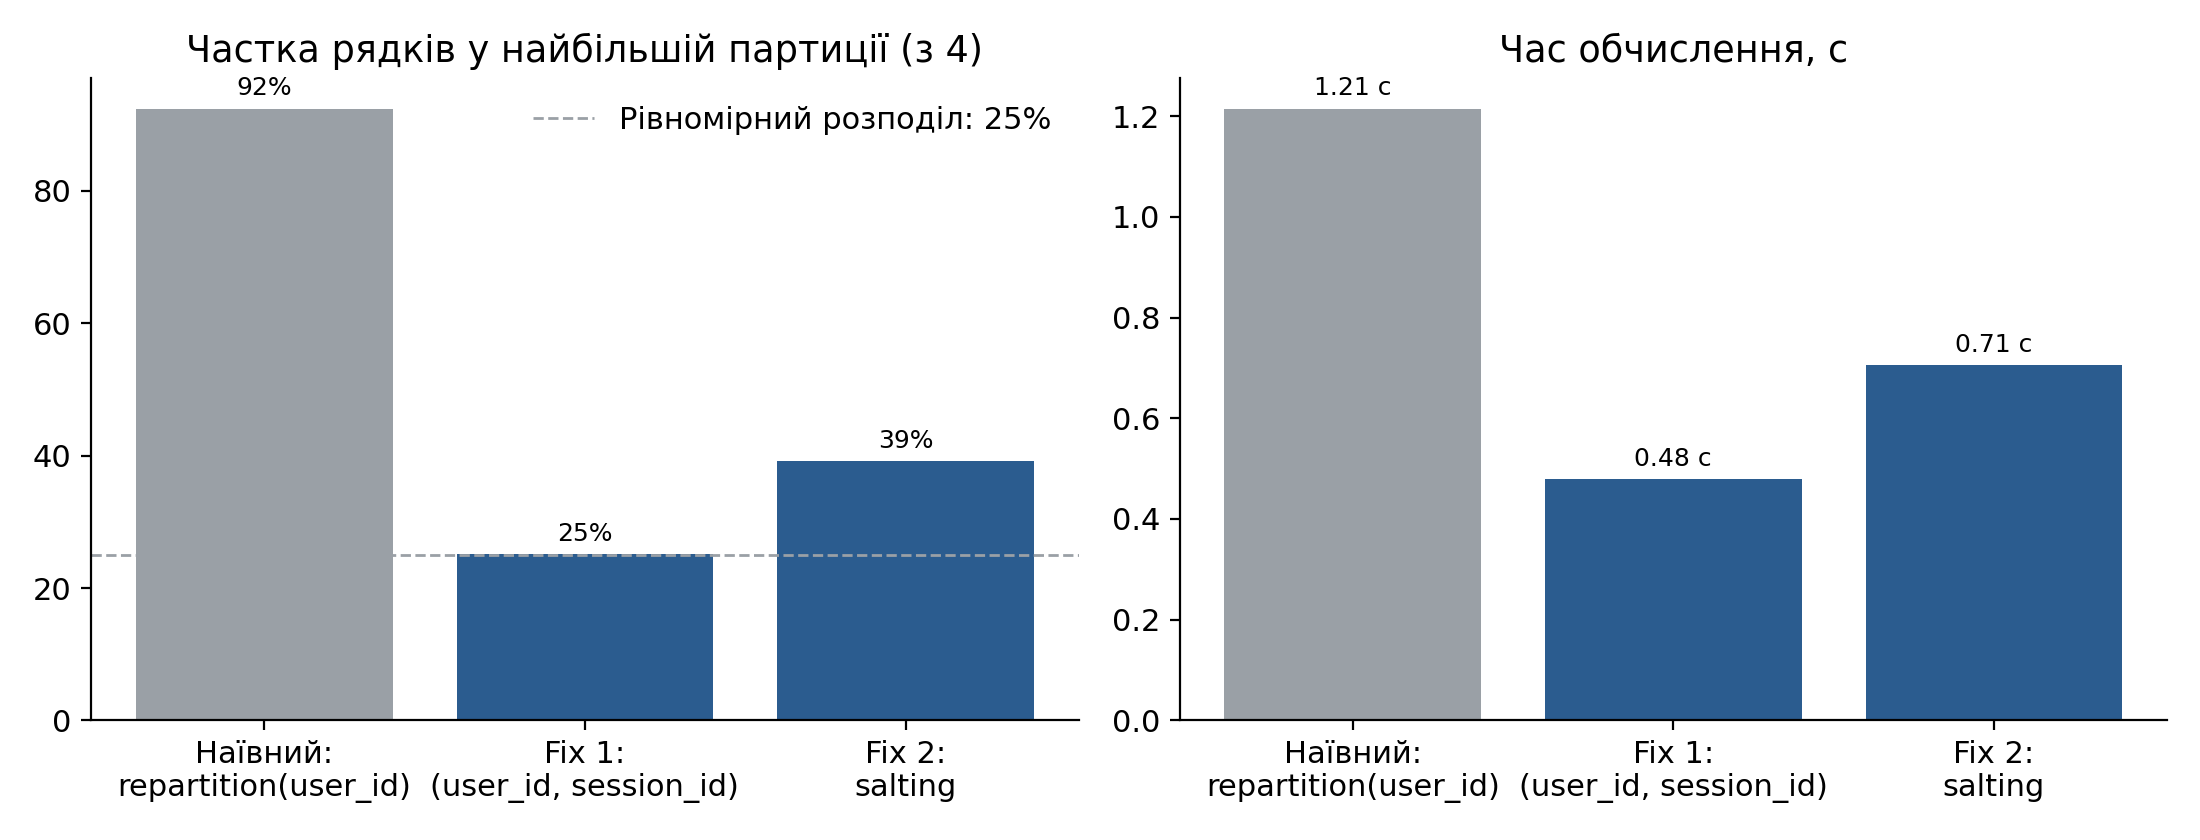
\includegraphics[width=0.85\textwidth]{lab4_skew.png}
\caption{Розподіл рядків між партиціями та час обчислення для перекошених даних}
\label{fig:skew}
\end{figure}

  Якщо розподіляти дані лише за \texttt{user\_id}, 92\% рядків потрапляють в одну партицію: одне ядро виконує майже всю роботу, а решта простоюють. За Амдалом це рівнозначно збільшенню послідовної частки до \(\approx 0.9\). Тому час зростає у 2.5 раза порівняно зі збалансованим варіантом. Способи пом'якшення:
  \begin{itemize}
    \item \emph{складений ключ} (\texttt{user\_id}, \texttt{session\_id}). Він і так є ключем групування, тож розподіл стає рівномірним (25.1\%, тобто ідеальні 25\%) без зміни логіки;
    \item \emph{salting}: до «гарячого» ключа додається сіль, тут \(\text{hash}(\texttt{session\_id}) \bmod 32\). Сіль обчислюється з \texttt{session\_id}, тому всі події однієї сесії отримують однакову сіль, і агрегація MAX\(-\)MIN залишається коректною за один крок. Для метрик на рівні користувача застосовується дво-етапна агрегація: спочатку за (\texttt{user\_id}, \texttt{salt}), потім за \texttt{user\_id};
    \item для з'єднань: \emph{AQE} (\texttt{spark.sql.adaptive.skewJoin.enabled}), окрема обробка «гарячих» ключів, broadcast малих таблиць.
  \end{itemize}
\end{enumerate}

\rsec{Висновки:} У ході виконання лабораторної роботи №4 засобами Apache Spark обчислено середню тривалість сесії (\(\approx 46.5\)~хв) для логу з 4.4 млн подій. Стратегія з примусовим round-robin перетасуванням (\texttt{repartition(200)}) виявилася в 6.8 раза повільнішою за розподіл за ключем групування з кількістю партицій, що дорівнює кількості ядер. Вона передає кожну подію мережею двічі (248 проти 98~MB shuffle) і створює 200 дрібних задач. Закон Амдала дав паралельну частку \(p \approx 0.91\) і граничне прискорення \(S_{\max} \approx 11\); вже на 8 ядрах ефективність знижується до 0.61. Перекіс, коли один користувач має 90\% сесій, видно за розміром партицій і задачами-«відстаючими». Розподіл лише за \texttt{user\_id} збирає 92\% даних в одній партиції та сповільнює обчислення в 2.5 раза, а розподіл за складеним ключем або salting усувають цю проблему. На реальному кластері, де перетасування йде через мережу, ці ефекти виражені ще сильніше.

\end{document}
